\section{Aggregation / 3-Way Join}
The correlation between CSC1015F course grades and Sakai usage is tested by investigating the correlation between the change in student's CSC1015F ranking compared to benchmarked ranking, and the count of each student's presense events (measured as logins to the Sakai system). The rationale is that the more often students log into Sakai, the more they are using it. This analysis shows how CouchDB could be used within a system designed to see the impact of greater Sakai LMS usage on CSC1015F grades.

\subsection{ETL}
Using nETL, rows are extracted from the three CSV files (\textit{Admissions (2014 - 2016).csv}, \textit{Grades (2014 - 2016).csv} and \textit{Events (2016).csv}) independently of each other and concurrently, in batches of 5 000, 10 000 and 30 000 rows respectively.

Via nETL configuration, rows from the admissions data are selected for students that are South African citizens or permanents residents, and that are in undergraduate; rows from the grades data are selected for students that attended CSC1015F during 2016 and as part of their undergraduate career; rows from the events data are selected for presence events only. Dynamic filters are configured for the admissions and events data to only include students that took the CSC1015F course.

The events data contains a field \textit{ref}, which is a long string and is not required in the analysis. As such, this string is dropped via a whitelisting process prior to serialization and loading strings into CouchDB (in batches via the \textit{\_bulk\_docs} endpoint). An example of a row from the event data serialized to a JSON string is shown in Figure \ref{fig-json-event}.

\begin{figure}[H]
    \centering
    \begin{mdframed}
        \centering
        \begin{minted}{text}
{
    "_id": "000e569ee321b915bae59fe62e0051e3",
    "_rev": "1-7112afce121087818c33ebfd0fd7fed7",
    "event_date": "2016-04-17T14:04:20.000Z",
    "event_id": 281, // anonymized student number
    "uct_id": 3018438,
    "site_key": 2297,
    "type_": "event"
}           
        \end{minted}
    \end{mdframed}
    \caption[Serialized events document]{\textbf{Figure \ref{fig-json-event}: Serialized events document}}
    \label{fig-json-event}
\end{figure}

\subsection{Index Calculation}
Since a single student may be associated with many rows in the Event data (sometimes even thousands of rows), a reduce function is used within the MapReduce job to aggregate the Events rows into a single document that is a count of Sakai presence events for first and second semester, with the output of this aggregation included in the index along with grade and benchmark data when reduce = true. The index consists of key:value pairs of student numbers associated a tuple that contains values for grades, benchmarks, and event information.

During map function execution, logical handling of the Grade and Benchmark entities is discussed previously. If the document is a line of the Events entity then the date of the event is categorized as either having occurred in semester 1 or semester 2. A key of [Student ID, 0, Year] is emitted along with the tuple [S1, S2]. The S1, and S2 (semester) variables are 0 by default, and depending on the date of the presence event, one of these variables is altered to be `1'. CSC1015F is a first semester course, but by including a count of both semester's it is possible use the same indexing code on courses that run in the second semester as well. Logic of the map function is shown in Figure \ref{fig-mapfn-correlation-events}.

Using the \_sum reduce function, an aggregation is done across all documents with the same key; this means that per a student, an aggregation is performed on a single Grade document, a single Benchmark document, and many Events documents in which the S1 and S2 variables are summed to form the tuple [sum of S1, sum of S2]. The key emitted for each type of entity is designed so that the view-index is ordered by StudentID. For each student number, documents are ordered by the second key (course), which means that Benchmarks and Events entities are sorted to be before grades for a student; and the \nth{3} component of each key results in benchmark data always being before Events documents. As such, during view-index retrieval it can be taken as given that for a single student ID, first documents of type Benchmark will be retrieved, followed by documents of type Event, followed by documents of type Grade.

\begin{sidewaysfigure}
    \centering
    \begin{mdframed}
        \centering
        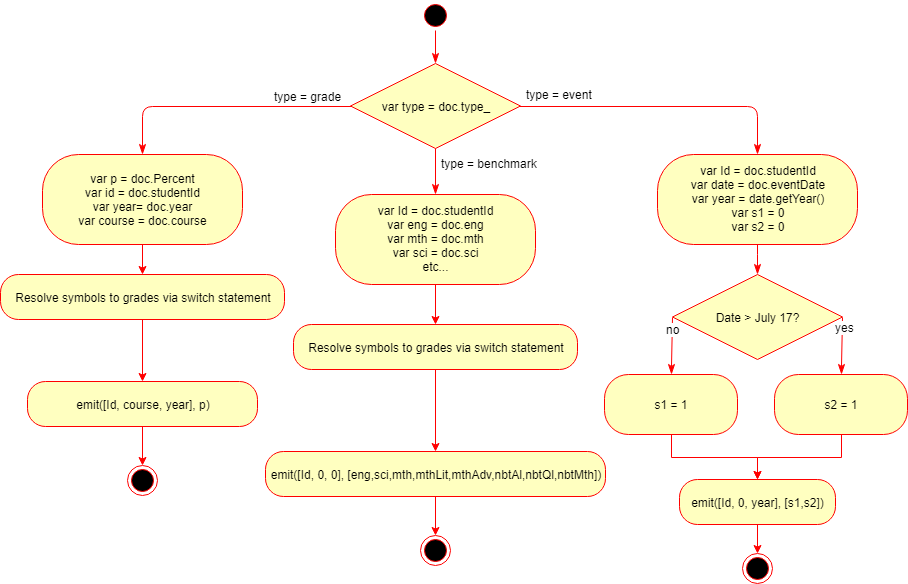
\includegraphics[scale=0.7]{./resources/figures/fig-mapfn-correlation-events.png}
    \end{mdframed}
    \caption[\textit{Map}-function: \texorpdfstring{(grades $\bowtie$ events) $\leftouterjoin$ admissions}{Lg}]{\textbf{Figure \ref{fig-mapfn-correlation-events}: \textit{Map}-function: \texorpdfstring{(grades $\bowtie$ events) $\leftouterjoin$ admissions}{Lg}}}
    \label{fig-mapfn-correlation-events}
\end{sidewaysfigure}


\subsection{Index Retrieval}
A list function implemented to retrieve the index with \mintinline{text}{reduce = true \& group = true} so that only reduced index output is retrieved, grouped by key.

Because the ranking of students for course grade and each benchmarking method is required, several ordered lists are kept in memory for the duration of a single course code is being processed (in this case CSC1015F). In other words, for each course code, and then for every result retrieved from the index, the student number of the row being processed is checked and compared to the student number of the previous row. If the current student number is not the same as the previous student number, then the current rows in memory are joined, list of ranks for each course and benchmark are updated. It is necessary to process all a index output for a particular course code before students can be ranked for a course (as well be ranked in terms of their benchmark placing compared to other students who took that course).

As joins are performed, an object is kept in memory for each student that keeps track of their course grade and scores for each benchmark. Once a single courses results have been iterated over, ranking lists are created that comprise tuples of [StudentId, \%] and are ordered by the second index ($i = 1$). The object of students is updated to add a delta value for (course \% - benchmark \%) (there is a delta value for each benchmark).

Then, by iterating over the student object it is possible to perform the summations stipulated in Equation \ref{eq:correlation}, and the correlation between $\Delta$ class rank and events count is found (a separate correlation corresponding to each benchmark is obtained).

List function logic is represented as an activity diagram in Figure \ref{fig-listfn-correlation-events}, and is configured to output a table of correlation coefficients for each benchmarking method as shown in Table \ref{tbl-correlation-events}.

\begin{figure}[H]
    \centering
    \begin{mdframed}
        \centering
        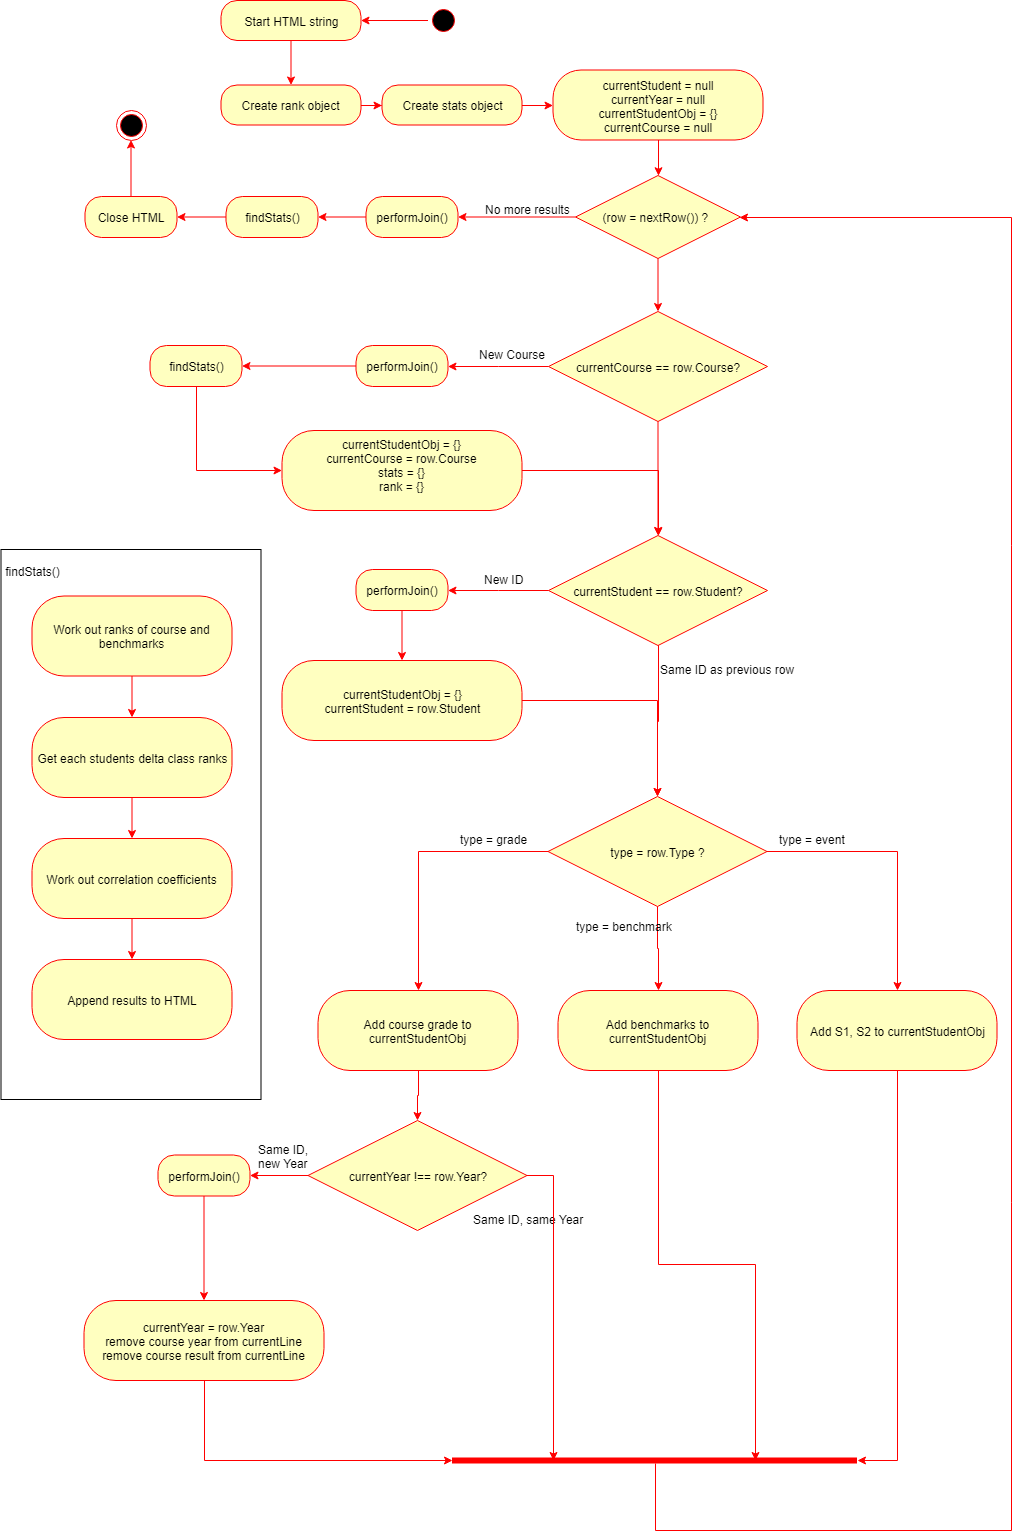
\includegraphics[scale=0.4]{./resources/figures/fig-listfn-correlation-events.png}
    \end{mdframed}
    \caption[\textit{List}-function: \texorpdfstring{(grades $\bowtie$ events) $\leftouterjoin$ admissions}{Lg}]{\textbf{\textit{List}-function: \texorpdfstring{(grades $\bowtie$ events) $\leftouterjoin$ admissions}{Lg}}}
    \label{fig-listfn-correlation-events}
\end{figure}



\begin{table}[H]
    \begin{threeparttable}
        \textbf{Table \ref{tbl-correlation-events}}\par\medskip\par\medskip
        \caption{Correlation Sakai presence and (course class rank - benchmark class rank)}
        \label{tbl-correlation-events}
        \begin{tabularx}{\textwidth}{>{\hsize=1.3\hsize}X>{\hsize=0.7\hsize}Y}
            \toprule
            \mC{c}{Benchmark}                     & \mC{c}{$r$} \\
            \midrule
            Gr12 Eng \%                           & 0.007       \\
            Gr12 Sci \%                           & -0.091      \\
            Gr12 Mth \%                           & -0.038      \\
            NBT AL \%                             & 0.144       \\
            NBT QL \%                             & 0.166       \\
            NBT Mth \%                            & 0.017       \\
            Avg Gr12 \%                           & -0.073      \\
            Avg Gr12 \% (Dbl Mth)                 & -0.070      \\
            Avg Gr12 \% (Dbl Mth \& Sci)          & -0.076      \\
            Avg NBT \%                            & 0.119       \\
            Avg NBT \% (Dbl AL)                   & 0.128       \\
            Avg NBT \% (Dbl QL)                   & 0.138       \\
            Avg NBT \% (Dbl Mth)                  & 0.087       \\
            Avg NBT \% (Dbl AL/QL)                & 0.141       \\
            Avg NBT \% (Dbl AL/Mth)               & 0.120       \\
            Avg NBT \% (Dbl QL/Mth)               & 0.111       \\
            Avg Gr12 \& NBT                       & 0.016       \\
            Avg Gr12 \& NBT (Dbl Gr12 Mth)        & -0.012      \\
            Avg Gr12 \& NBT (Dbl Gr12 Mth \& Sci) & -0.048      \\
            \bottomrule
        \end{tabularx}
    \end{threeparttable}
\end{table}